% Framework overview for Chapter 1 and the presentation.
% Drawn at about 24 cm wide in 10pt type so that, placed at \textwidth (16 cm), text prints at
% about 6.7pt. The braces on the right mark the three loci of control; output lies outside them.
% Build: pdflatex fig1-1-framework-overview.tex
%        pdftoppm -png -r 300 -singlefile fig1-1-framework-overview.pdf ../fig1-1-framework-overview
\documentclass[tikz,border=3pt]{standalone}
\usepackage[T1]{fontenc}
\usepackage{helvet}
\renewcommand{\familydefault}{\sfdefault}
\usetikzlibrary{shapes.geometric,arrows.meta,decorations.pathreplacing}

\definecolor{cblue}{HTML}{2F5597}
\definecolor{cbluefill}{HTML}{EAF1FB}
\definecolor{cgreen}{HTML}{2E7D4F}
\definecolor{cgreenfill}{HTML}{EAF6EE}
\definecolor{cpurple}{HTML}{6B4FA3}
\definecolor{cpurplefill}{HTML}{F1EDF9}
\definecolor{cred}{HTML}{B23A48}
\definecolor{credfill}{HTML}{FBEDEF}
\definecolor{corange}{HTML}{C8691A}
\definecolor{cgrey}{HTML}{6B7280}
\definecolor{ctext}{HTML}{374151}

\tikzset{
  card/.style 2 args={draw=#1, fill=#2, rounded corners=3pt, line width=0.8pt,
    align=center, inner sep=0.14cm},
  flow/.style={-{Stealth[length=6pt]}, line width=0.8pt},
  every node/.style={execute at begin node={\hyphenpenalty=10000\exhyphenpenalty=10000}},
}

\newcommand{\cardtext}[2]{\textbf{#1}\\[2pt]{\color{ctext}#2}}

\begin{document}
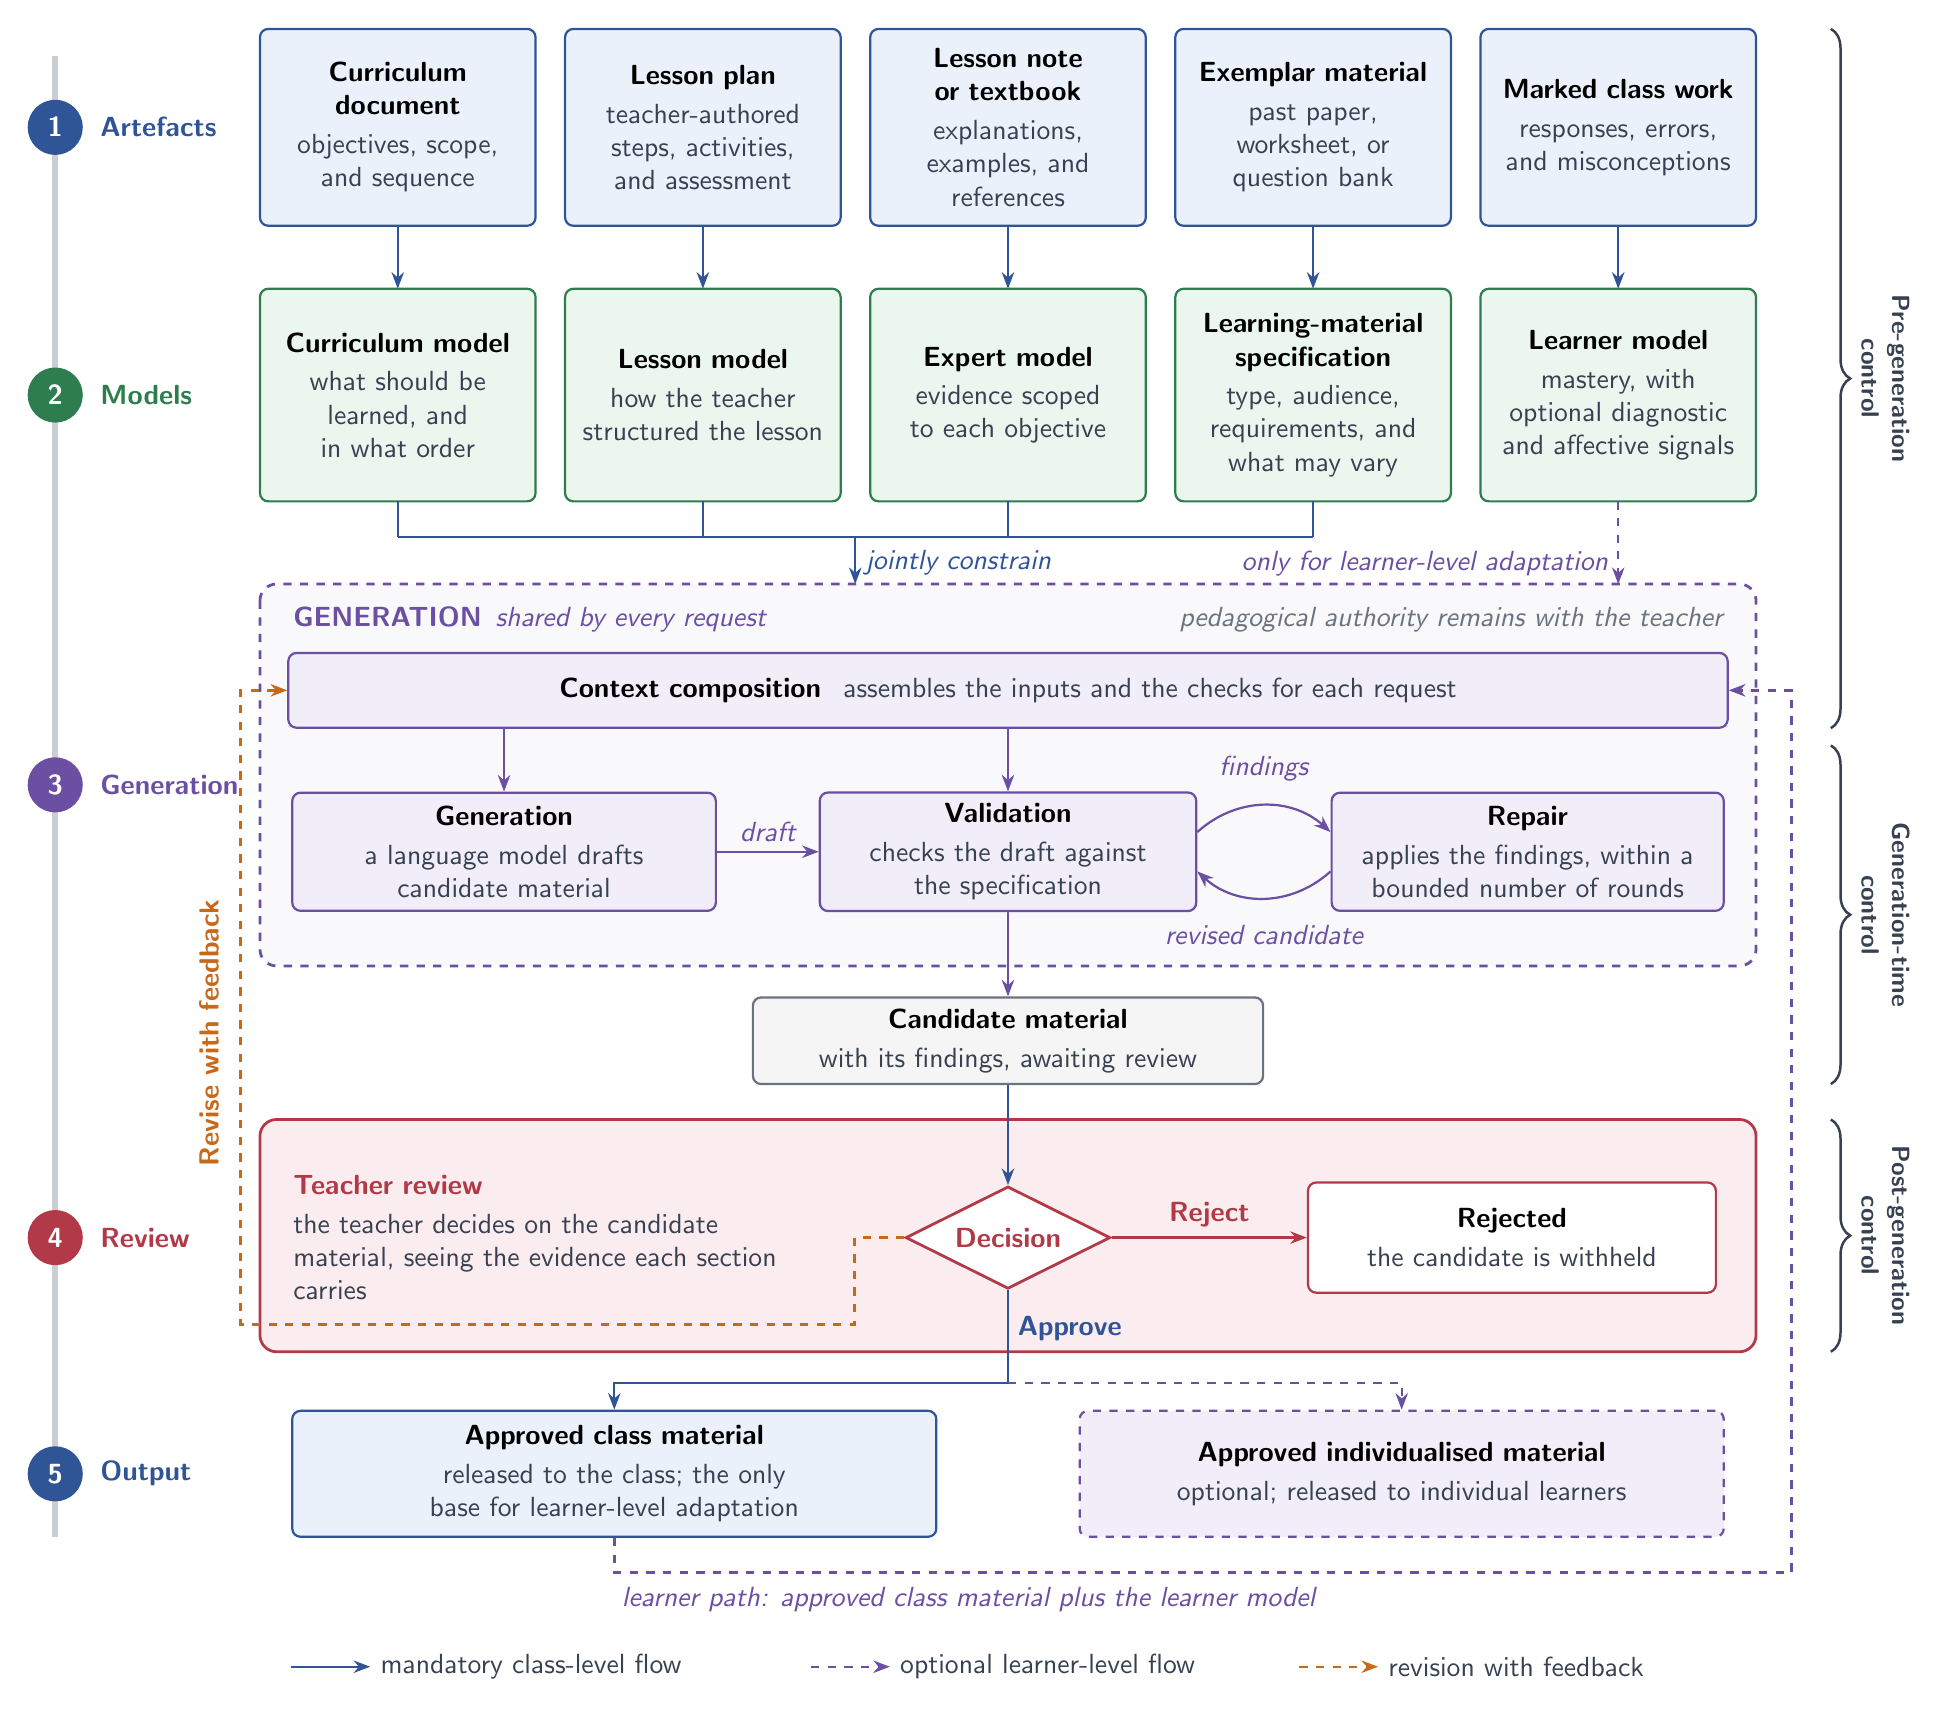
\begin{tikzpicture}

% band rail
\draw[cgrey!35, line width=2pt] (0.4,0.9) -- (0.4,-17.9);
\foreach \y/\n/\t/\c in {0/1/Artefacts/cblue, -3.4/2/Models/cgreen, -8.35/3/Generation/cpurple, -14.1/4/Review/cred, -17.1/5/Output/cblue} {
  \node[circle, fill=\c, text=white, font=\bfseries, minimum size=0.7cm, inner sep=0pt] at (0.4,\y) {\n};
  \node[anchor=west, font=\bfseries, text=\c] at (0.85,\y) {\t};
}

% band 1: existing artefacts
\foreach \x/\a/\b in {
  4.75/{Curriculum document}/{objectives, scope, and sequence},
  8.625/{Lesson plan}/{teacher-authored steps, activities, and assessment},
  12.5/{Lesson note or textbook}/{explanations, examples, and references},
  16.375/{Exemplar material}/{past paper, worksheet, or question bank},
  20.25/{Marked class work}/{responses, errors, and misconceptions}} {
  \node[card={cblue}{cbluefill}, text width=3.22cm, minimum height=2.5cm] at (\x,0) {\cardtext{\a}{\b}};
  \draw[flow, cblue] (\x,-1.25) -- (\x,-2.05);
}

% band 2: structured models
\foreach \x/\a/\b in {
  4.75/{Curriculum model}/{what should be learned, and in what order},
  8.625/{Lesson model}/{how the teacher structured the lesson},
  12.5/{Expert model}/{evidence scoped to each objective},
  16.375/{Learning-material specification}/{type, audience, requirements, and what may vary},
  20.25/{Learner model}/{mastery, with optional diagnostic and affective signals}} {
  \node[card={cgreen}{cgreenfill}, text width=3.22cm, minimum height=2.7cm] at (\x,-3.4) {\cardtext{\a}{\b}};
}
\foreach \x in {4.75,8.625,12.5,16.375} { \draw[cblue, line width=0.8pt] (\x,-4.75) -- (\x,-5.2); }
\draw[cblue, line width=0.8pt] (4.75,-5.2) -- (16.375,-5.2);
\draw[flow, cblue] (10.56,-5.2) -- (10.56,-5.8) node[pos=0.55, right, font=\itshape, text=cblue] {jointly constrain};
\draw[flow, cpurple, dashed] (20.25,-4.75) -- (20.25,-5.8) node[pos=0.75, left, font=\itshape, text=cpurple] {only for learner-level adaptation};

% band 3: generation harness
\draw[cpurple, dashed, rounded corners=6pt, line width=1pt, fill=cpurple!4] (3.0,-5.8) rectangle (22.0,-10.65);
\node[anchor=west, text=cpurple] at (3.3,-6.25) {\textbf{GENERATION}\hspace{0.5em}\itshape shared by every request};
\node[anchor=east, text=cgrey, font=\itshape] at (21.7,-6.25) {pedagogical authority remains with the teacher};
\node[card={cpurple}{cpurplefill}, text width=18cm, minimum height=0.95cm] (cc) at (12.5,-7.15)
  {\textbf{Context composition}\hspace{0.8em}{\color{ctext}assembles the inputs and the checks for each request}};
\node[card={cpurple}{cpurplefill}, text width=5.1cm, minimum height=1.5cm] (gen) at (6.1,-9.2)
  {\cardtext{Generation}{a language model drafts candidate material}};
\node[card={cpurple}{cpurplefill}, text width=4.5cm, minimum height=1.5cm] (val) at (12.5,-9.2)
  {\cardtext{Validation}{checks the draft against the specification}};
\node[card={cpurple}{cpurplefill}, text width=4.7cm, minimum height=1.5cm] (rep) at (19.1,-9.2)
  {\cardtext{Repair}{applies the findings, within a bounded number of rounds}};
\draw[flow, cpurple] (6.1,-7.625) -- (gen.north);
\draw[flow, cpurple] (12.5,-7.625) -- (val.north);
\draw[flow, cpurple] (gen.east) -- (val.west) node[midway, above, font=\itshape, text=cpurple] {draft};
\draw[flow, cpurple] (val.east |- 0,-8.95) .. controls (15.4,-8.5) and (16.1,-8.5) .. (rep.west |- 0,-8.95);
\draw[flow, cpurple] (rep.west |- 0,-9.45) .. controls (16.1,-9.9) and (15.4,-9.9) .. (val.east |- 0,-9.45);
\node[font=\itshape, text=cpurple] at (15.75,-8.15) {findings};
\node[font=\itshape, text=cpurple] at (15.75,-10.25) {revised candidate};

% candidate material
\node[card={cgrey}{black!4}, text width=6.2cm, minimum height=1.1cm] (cand) at (12.5,-11.6)
  {\cardtext{Candidate material}{with its findings, awaiting review}};
\draw[flow, cpurple] (val.south) -- (cand.north);

% band 4: teacher review
\draw[cred, rounded corners=6pt, line width=1pt, fill=credfill] (3.0,-12.6) rectangle (22.0,-15.55);
\node[anchor=west, text width=6.4cm, align=left] at (3.3,-14.1)
  {{\color{cred}\textbf{Teacher review}}\\[2pt]{\color{ctext}the teacher decides on the candidate material, seeing the evidence each section carries}};
\node[diamond, aspect=2.2, draw=cred, fill=white, line width=1pt, minimum width=2.6cm, minimum height=1.3cm, inner sep=1pt, font=\bfseries, text=cred] (dec) at (12.5,-14.1) {Decision};
\draw[flow, cblue] (cand.south) -- (dec.north);
\node[card={cred}{white}, text width=4.9cm, minimum height=1.4cm] (rej) at (18.9,-14.1)
  {\cardtext{Rejected}{the candidate is withheld}};
\draw[flow, cred] (dec.east) -- (rej.west) node[midway, above, font=\bfseries, text=cred] {Reject};
\draw[flow, corange, dashed, line width=1pt] (dec.west) -- (10.55,-14.1) -- (10.55,-15.2) -- (2.75,-15.2) -- (2.75,-7.15) -- (cc.west);
\node[rotate=90, anchor=south, font=\itshape\bfseries, text=corange] at (2.6,-11.5) {Revise with feedback};

% band 5: approved output
\draw[cblue, line width=0.8pt] (dec.south) -- (12.5,-15.95);
\node[right, font=\bfseries, text=cblue] at (12.5,-15.25) {Approve};
\node[card={cblue}{cbluefill}, text width=7.9cm, minimum height=1.6cm] (cls) at (7.5,-17.1)
  {\cardtext{Approved class material}{released to the class; the only base for learner-level adaptation}};
\node[card={cpurple}{cpurplefill}, dashed, text width=7.9cm, minimum height=1.6cm] (ind) at (17.5,-17.1)
  {\cardtext{Approved individualised material}{optional; released to individual learners}};
\draw[flow, cblue] (12.5,-15.95) -| (cls.north);
\draw[flow, cpurple, dashed] (12.5,-15.95) -| (ind.north);
\draw[flow, cpurple, dashed, line width=1pt] (cls.south) -- (7.5,-18.35) -- (22.45,-18.35) -- (22.45,-7.15) -- (cc.east);
\node[font=\itshape, text=cpurple] at (12.0,-18.7) {learner path: approved class material plus the learner model};

% loci of control: pre-generation spans artefacts, models and context composition; generation-time
% spans generation, validation, repair and the candidate; post-generation is teacher review.
\foreach \top/\bot/\locus in {1.25/-7.63/Pre-generation, -7.85/-12.15/Generation-time,
                              -12.6/-15.55/Post-generation} {
  \draw[decorate, decoration={brace, amplitude=7pt}, line width=0.9pt, ctext] (22.95,\top) -- (22.95,\bot);
  \node[rotate=-90, anchor=south, align=center, font=\small\bfseries, text=ctext, inner sep=1pt]
    at (23.3,{(\top+\bot)/2}) {\locus\\control};
}

% legend
\draw[flow, cblue] (3.4,-19.55) -- (4.4,-19.55) node[right, text=ctext] {mandatory class-level flow};
\draw[flow, cpurple, dashed] (10.0,-19.55) -- (11.0,-19.55) node[right, text=ctext] {optional learner-level flow};
\draw[flow, corange, dashed] (16.2,-19.55) -- (17.2,-19.55) node[right, text=ctext] {revision with feedback};

\end{tikzpicture}
\end{document}
